\documentclass[conference]{IEEEtran}
\IEEEoverridecommandlockouts
% The preceding line is only needed to identify funding in the first footnote. If that is unneeded, please comment it out.
\usepackage{cite}
\usepackage{amsmath,amssymb,amsfonts}
\usepackage{algorithmic}
\usepackage{graphicx}
\usepackage{textcomp}
\usepackage{xcolor}
\def\BibTeX{{\rm B\kern-.05em{\sc i\kern-.025em b}\kern-.08em
    T\kern-.1667em\lower.7ex\hbox{E}\kern-.125emX}}
\begin{document}

\title{Dynamic Load Balancing for Particle-in-Cell, CFD, and Discrete Event Simulations\\
\thanks{Identify applicable funding agency here. If none, delete this.}
}

\author{\IEEEauthorblockN{1\textsuperscript{st} Gerrett Diamond}
\IEEEauthorblockA{\textit{SCOREC} \\
\textit{Rensselaer Polytechnic Institute}\\
Troy, NY\\
diamog@rpi.edu}
\and
\IEEEauthorblockN{2\textsuperscript{nd} Cameron W. Smith}
\IEEEauthorblockA{\textit{SCOREC} \\
\textit{Rensselaer Polytechnic Institute}\\
Troy, NY\\
smithc11@rpi.edu}
\and
\IEEEauthorblockN{3\textsuperscript{rd} Mark S. Shephard}
\IEEEauthorblockA{\textit{SCOREC} \\
\textit{Rensselaer Polytechnic Institute}\\
Troy, NY\\
shephard@rpi.edu}
}

\maketitle

\begin{abstract}

\end{abstract}

\begin{IEEEkeywords}
component, formatting, style, styling, insert
\end{IEEEkeywords}

\section{Introduction}

\begin{itemize}
\item motivate dynamic load balancing
\item talk about how different applications have different partitioning needs
\item Mention that engpar is general to support a range of structures.
\end{itemize}

\section{EnGPar}

\begin{itemize}
%\item Discuss the Ngraph in general graph terms with some figures
\item Discuss the construction for a element-partitioned mesh as an example with figure
%\item Discuss dynamic load balancing and the general diffusive steps
\end{itemize}

EnGPar is a tool for partition improvement and dynamic load balancing. EnGPar
utilizes a multi-hypergraph, called the N-graph, to represent the data of an
application in a relational format that allows load balancing of the vertices
and edges simultaneously. The N-graph is defined as $G^n = \{V, H^n, P^n\}$ where
$V$ is the set of vertices in the graph. The vertices are uniquely owned by a single
process and are used to represent the main source of data in an application.
$H^n = \{H_1, ..., H_n\}$ are sets of hyperedges where each hyperedge connects a
subset of vertices in $V$. The pins, $P^n = \{P_1,...,P_n\}$, represent the connections from
vertices to hyperedges. Each application that utilizes EnGPar represents the data
that needs partitioning as an N-graph before running any of the partitioning tools.
The general design of the N-graph allows easy representation for different applications
that use structures such as meshes, graphs, and other relational structures.

%Add an example of constructing the n-graph

EnGPar's partition improvement is driven by local diffusive techniques that migrate weight
from heavily weighted parts to lightly weighted parts. This is done by iteratively running
a set of steps until the target imbalance is met or no further improvements can be met.
A diffusive iteration consists of three steps: targeting, selection, and migration.
The targeting step consists of gathering information about the current partiton and deciding
which neighbors should be sent weight and how much weight to send. The selection step constructs
a plan of what vertices should be sent to each neighbor in order to satisfy the weights in
the targeting step. The final step, migration, is where the vertices are sent to their
destinations and the partition is changed.

\section{Particle In Cell}

\begin{itemize}
\item Briefly discuss PIC/XGCM
\item Mention that the mesh partition is static.
\item Describe the buffer/safe zone
\item Describe the weight diffusion algorithm.
\end{itemize}

Since the mesh partitions in XGCM are fixed based on the geometry, we only consider
load balancing the particles. The main consideration when migrating particles in XGCM
is that a particle must always be in an element that is in the safe zone of a part.
This means that if a particle moves outside the safe zone, it must be migrated to a
new process where it is safe and when load balancing particles we must ensure that every
particle is migrated to a process where it is in the safe zone of the part.

To handle both cases, we construct the N-graph carefully such that any partition
decision in EnGPar will always maintain this requirement in XGCM. First we define
the components of XGCM by the following: {\color{red} Probably should turn these lists
  into full text instead.}
\begin{itemize}
\item Let $F = \{F_1,F_2, ..., F_n\}$ be the flux faces.
\item Let $G = \{G_1, G_2, ..., G_n\}$ be the groups such that $G_i$
  contains $F_i$ and the suitable buffer region around $F_i$
\item Let $S = \{S_1,S_2,...,S_n\}$ be the safe zones for each $G_i$.
  It is required that $S_i \subset G_i$.
\item Define $\bar{S_j}$ for each set of overlapping safe zones.
\item Let $P$ be the set of particles.
\item For each particle $p\in P$, Let $T_p$ be the set of safe zones in $S$ that $p$ resides
  in.  $\forall p \in P, \exists ! i$ such that $T_p = \bar{S_i}$.
\item  Let $P_{\bar{S_i}}$ be the set of particles such that $\forall p \in P_{\bar{S_i}}, T_p = \bar{S_i}$.
\end{itemize}

With these definitions, we define the Ngraph as $G = \{V, H, P\}$ where:
\begin{enumerate}
\item $V = \{ v_{i,j}$ for each $\bar{S_i} | S_j \in \bar{S_i} \}$.
\item The weight of vertex $v_{t,i}$ is equal to $|P_{\bar{S_i}}|$ on process $t$.
\item $H = \{ h_i$ for each $\bar{S_i} \}$.
\item $P = \{ p_{i,j}$ connecting $v_{i,j}$ to $h_i \}$.
\end{enumerate}
Figure \ref{fig:sbars} shows an example of the $\bar{S_i}$ and the construction of N-graph from
them. {\color{red} Make example figure smaller so it is visible in paper.}

\begin{figure}[!ht]
  \centering
  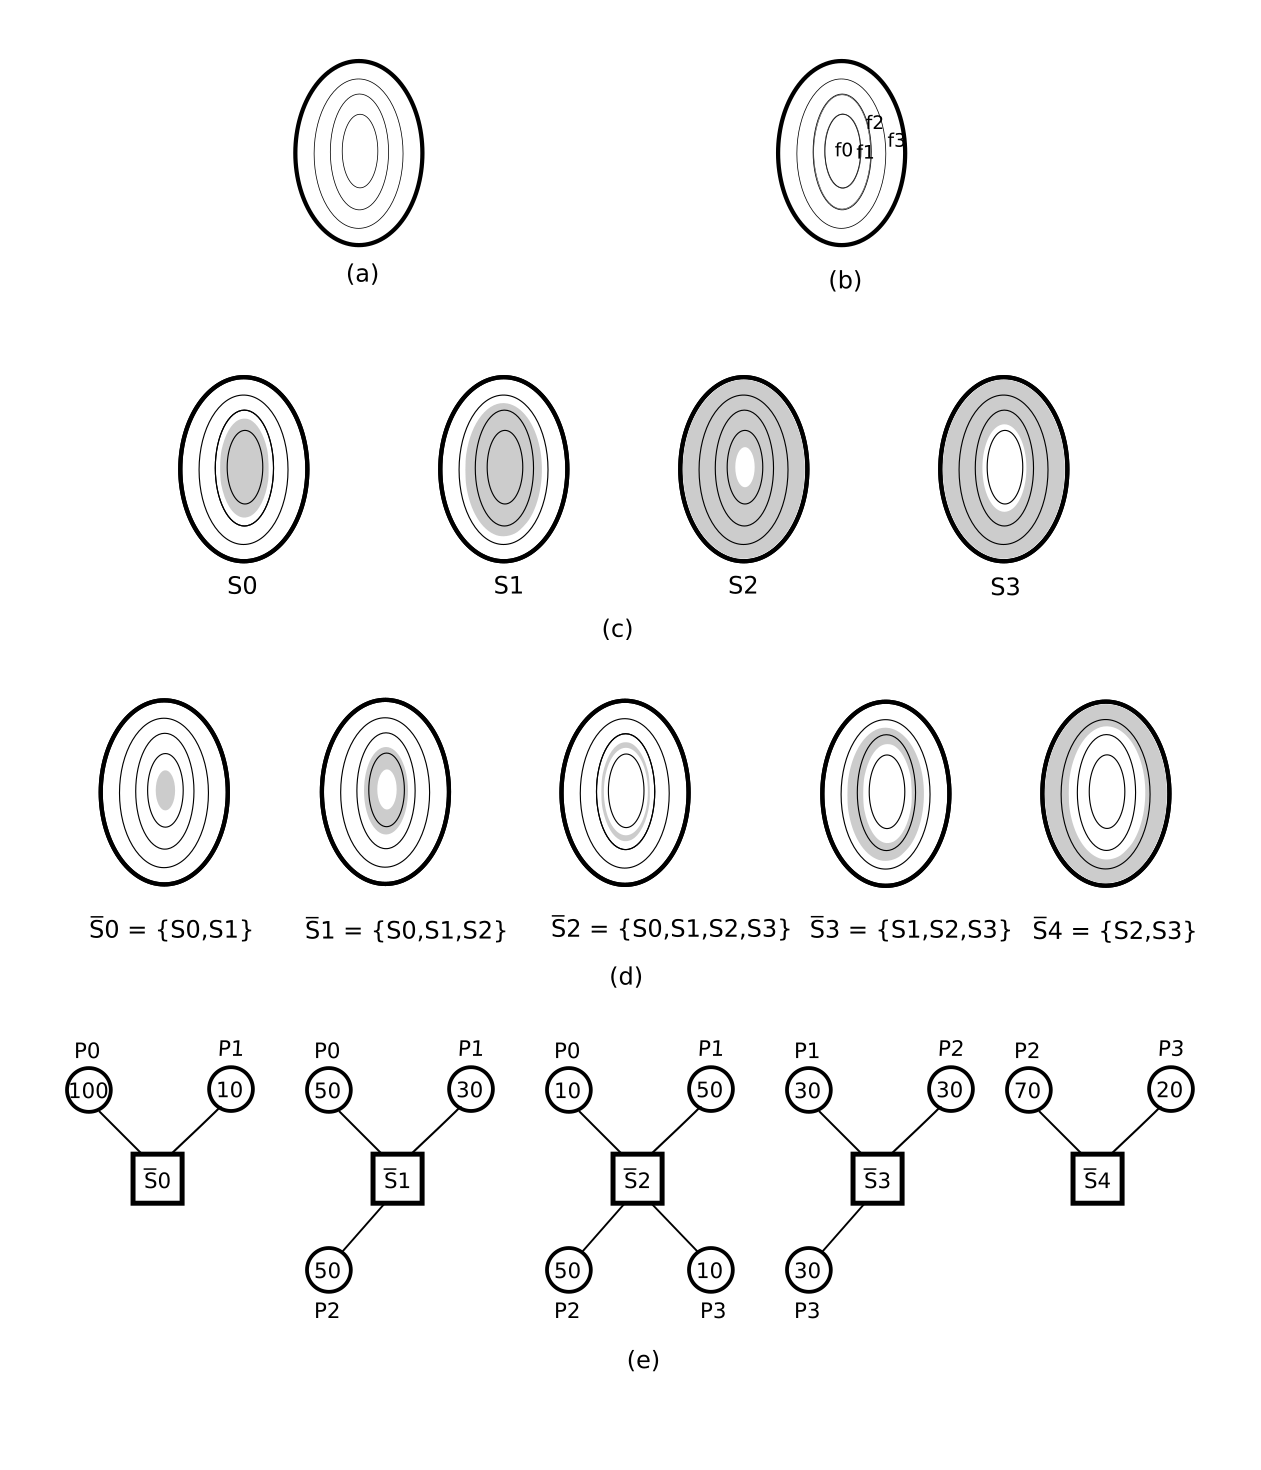
\includegraphics[width=.4\textwidth]{../figures/xgcm_ngraph_construction.png}
  \caption{An example of overlapping safe zones and the N-graph constructed from them.}
  \label{fig:sbars}
\end{figure}

In order to load balance this graph, we run diffusive techniques on the weights of the vertices
rather than the vertices. This means that instead of migrating graph vertices, we migrate the
weight of the vertices across hyperedges to reduce the imbalance of load in the graph.

\begin{itemize}
\item Add particle selection after engpar.
\item Add results of using engpar vs not using engpar
\item Add timing results compared to an iteration of XGCM.
\end{itemize}

\section{Computational Fluid Dynamics}

\begin{itemize}
\item Briefly discuss CFD (FUN3D).
%\item Discuss vertex-based partition vs. element-based partition.
%\item Discuss how EnGPar/Ngraph can support vertex partitions.
\item Discuss the current approach in FUN3D for partitioning and our ideas to improve it.
\item Mention the boundary stack and our approach to better represent it.
\end{itemize}


To represent the vertex-partitioned mesh in EnGPar, the construction
is essentially the opposite of the element-partitioned mesh. Graph
vertices are defined by mesh vertices and graph hyperedges are defined
by mesh elements. The pins between graph vertices and hyperedges are
created for any mesh vertex that bounds a mesh element.
{\color{red} The following line can be removed if we don't do this.}
Additionally, a second edge type is used for mesh edges where each
hyperedge would have pins to the two mesh vertices that bound the mesh edge.

{\color{red} Add a figure of vertex-partitioned mesh to Ngraph?}

Currently for the application, partitioning is done by running (Par)METIS on the graph created
from mesh vertices and mesh edges. As normally seen from multilevel graph
partitioning [REFERENCES],
the vertices are partitioned well, but the mesh edges and mesh elements have a large
imbalance which are key components of the computational load.

During initial attempts at improving the partitions, we found that the edge cut was growing
at a large rate as we improved edge imbalance. This has been attributed to the differences
caused by the vertex-partitioning of the mesh. For element-partitioned meshes, the hyperedges
represent the mesh vertices. To maintain a low edge cut, mesh vertices that bound many mesh
elements should not be cut across partitions. Towards this, EnGPar avoids migrating cavities
around these high-degree hyperedges. For vertex-partitioned meshes, this problem is reveresed
since mesh vertices are represented as graph vertices and hyperedges all have roughtly uniform
low degrees based on the element: four in a tetrahedron, five in a pyramid, six in a prism, etc.
Thus the problem of edge cut arises for having high degree graph vertices along the partition
boundary which leads to a larger edge cut.

To control the edge cut while balancing the graph, we introduce a metric to represent the
potential edge cut change for a cavity. The metric is the ratio of hyperedges that will be cut
after the cavity is migrated to the hyperedges currently cut around the cavity. We introduce a
parameter to EnGPar that will only migrate a cavity if the metric is below the given tolerance.
Setting this parameter to 1.0 forces EnGPar to migrate cavities that will not increase the edge
cut. However, smaller values of this paramter will limit EnGPar's ability to improve the
imbalance and either take more iterations to reach the imbalance tolerance or stagnate at a
higher imbalance.



\section{Results}

\begin{itemize}
\item Compare parmetis graph partitions vs. Zoltan hypergraph partitions
\item Then compare how EnGPar can balance each.
\item Use FUN3D runs to compare how different metrics affect the runtime.
\end{itemize}


\section{Future Works}

\begin{itemize}
\item accelerators
\item Other ideas for load balancing vertex-based partitions?
\end{itemize}

{\color{red} Add bibliography stuff here}

\end{document}
